% !TeX encoding = UTF-8
% !TeX root = ../main.tex

%% ------------------------------------------------------------------------
%% Copyright (C) 2021 SJTUG
%% 
%% SJTUBeamer Example Document by SJTUG
%% 
%% SJTUBeamer Example Document is licensed under a
%% Creative Commons Attribution-NonCommercial-ShareAlike 4.0 International License.
%% 
%% You should have received a copy of the license along with this
%% work. If not, see <http://creativecommons.org/licenses/by-nc-sa/4.0/>.
%% -----------------------------------------------------------------------

\section{Security issues: privacy}

\subsection{Provenance of data}

\begin{frame}{Provenance of data}
  \begin{exampleblock}{Model updates}
  A blockchain-based privacy-preserving federated learning framework leverages the immutability and decentralized trust properties of blockchain to provide the \alert{provenance of model updates} \textbf{(smart contracts)}
%  \item \textbf{Benefit:} improved data collection efficiency and reduced costs effectively
  \end{exampleblock}
  \begin{figure}[h]
        \centering
        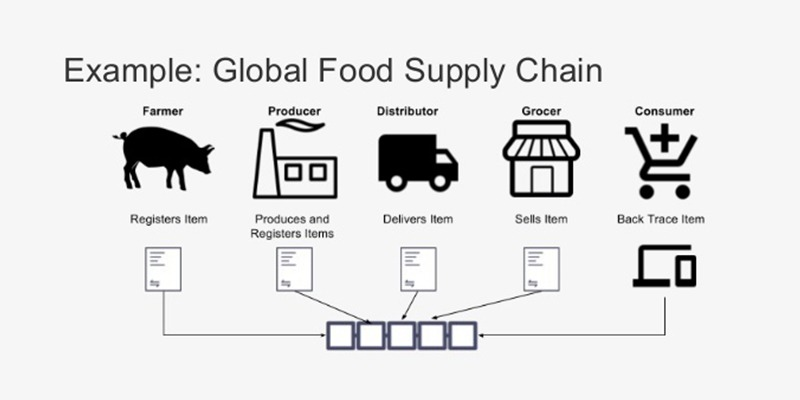
\includegraphics[width=.7\textwidth]{blockchain-in-supply-chain-industry-6.jpg}
      \end{figure}
\end{frame}

\subsection{Data privacy}

\begin{frame}{Data privacy}
\textbf{Improving data privacy in FL scenario:} 
\begin{itemize}
  		\item \alert{Storing evidence:} by using hashing and fingerprint mechanisms, references can be stored proving both local data and models are correct
  		\item \alert{Limiting access:} by making the ledger network only accessible via private network of participants
  		\item \alert{Zero Knowledge Proofs:} advanced (and computationally expensive) cryptographical techniques for granular information disclosure (both for mutual verification and partial data disclosure) 
\end{itemize}
\end{frame}

\section{Quality management: incentive}

\subsection{Incentive mechanism}

\begin{frame}{Incentive mechanism}
  \begin{exampleblock}{Federated Learning scenario}
 An effective incentive mechanism \alert{combining reputation with contract theory} motivates high-reputation mobile devices with high-quality data to participate in model learning
%  \item \textbf{Benefit:} improved data collection efficiency and reduced costs effectively
  \end{exampleblock}
  \begin{figure}[h]
        \centering
        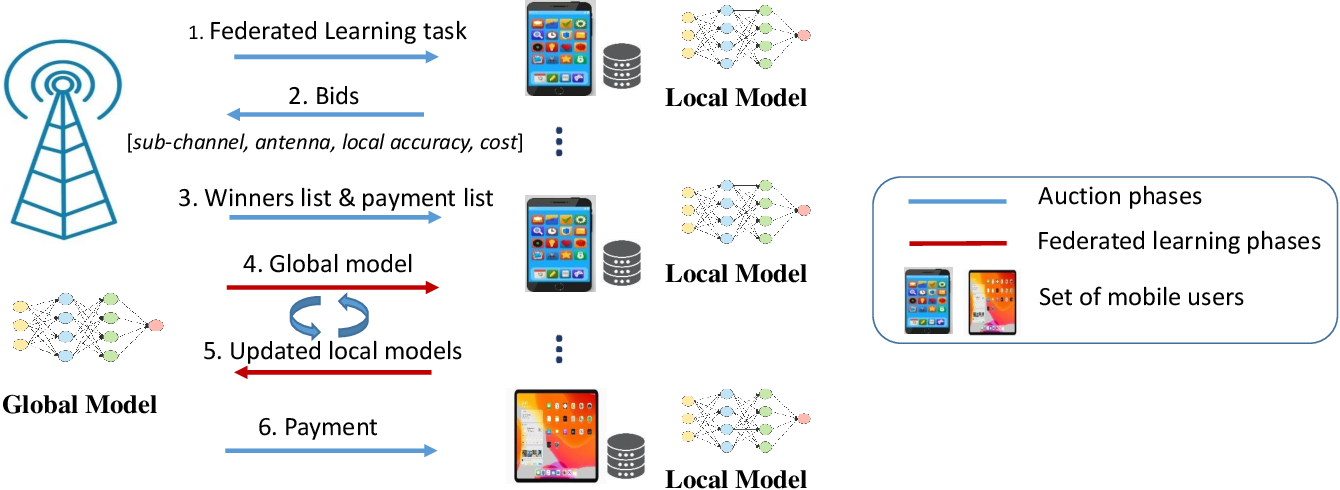
\includegraphics[width=.7\textwidth]{incentive-FL.png}
      \end{figure}
\end{frame}

%\subsection{1st research question}
%
%\begin{frame}{1st research question}
%	\begin{itemize}[<+- | alert@+>]
%		\item What are the differences between the use of standard networks and the use of
%blockchain networks in student mobility management in relation to the
%administration process efficiency?
%%		\metroset{block=fill}
%
%      \begin{block}{Goal}
%        Study the effects of blockchain technology in the field of student mobility
%management
%      \end{block}
%
%      \begin{block}{Methodology}
%        \emph{Quantitative:} Users activity logging (with and without blockchain)
%      \end{block}
%
%      \begin{block}{Analysis}
%        Social Network Analysis \& Web usage mining (logging)
%      \end{block}
%	\end{itemize}
%\end{frame}
%
%\subsection{2nd research question}
%
%\begin{frame}{2nd research question}
%	\begin{itemize}[<+- | alert@+>]
%		\item Following your paper on incentive model for crowdsensing\cite{electronics9020215}, I would like to explore how to use \alert{auction theory} and \alert{mechanism design theory} in a blockchain system, in order to identify an efficient model to assign exchange students to host universities (substituting classical competitive calls and applications).
%%		\metroset{block=fill}
%
%      \begin{block}{Goal}
%        Analyse the impact in student mobility competitive
%calls and applicants management
%      \end{block}
%
%      \begin{block}{Methodology}
%        \emph{Quantitative:} Several model simulations
%      \end{block}
%
%      \begin{block}{Analysis}
%        Effectiveness? Measure performance of several models
%      \end{block}
%	\end{itemize}
%\end{frame}
%
%\subsection{3rd research question}
%
%\begin{frame}{3rd research question}
%	\begin{itemize}[<+- | alert@+>]
%		\item Inter-universities agreements for student mobilites can be seen as a supply chain network: exchange students as assets. How to use \alert{machine learning} and \alert{predictive analytics} model, in a blockchain system, for better associations? Conflicts (geopolitical, pandemias, transport) alter mobilities feasibility. Effective planning?
%%		\metroset{block=fill}
%
%      \begin{block}{Goal}
%        Build a predictive model for optimal student mobility agreements
%      \end{block}
%
%      \begin{block}{Methodology}
%        \emph{Quantitative:} ratio of accomplished and failed mobilities
%      \end{block}
%
%      \begin{block}{Analysis}
%        Effectiveness? Measure performance of model in several scenarios
%      \end{block}
%	\end{itemize}
%\end{frame}

\subsection{Mechanism design: multifactor}

\begin{frame}{Mechanism design: multifactor}
  \begin{itemize}
    \item Based on three parameters:
          \begin{enumerate}
            \item \alert{Workers' bidding}
            \item \alert{Reputation}
            \item \alert{Recent data quality estimation}
          \end{enumerate}
    \item Analytic Hierarchy Process (AHP) framework \rightarrow (top-down)
    	\begin{enumerate}
            \item \alert{Objective level}: winning workers
            \item \alert{Criteria level}: parameters criteria
            \item \alert{Alternative level}: workers available
          \end{enumerate}
    \end{itemize}
    \begin{exampleblock}{Multifactor worker evaluation approach}
    	\begin{equation*}
      	\theta_{i}=\omega_{1} B_{i}+\omega_{2} R_{i}+\omega_{3} Q_{i} \quad\quad \text { where } \omega_{i} \geq 0 \text { and } \sum_{\omega_{i}=1}^{3} \omega_{i}=1	
    	\end{equation*}
  \end{exampleblock}
\end{frame}

\subsection{Mechanism design: issues}

\begin{frame}{Mechanism design: issues}
  		\begin{enumerate}
   			\item \textbf{How to select appropriate workers?}
   				\begin{itemize}
   					\item \textbf{Proposal: } decentralized architecture (blockchain technology) that lacks a single point of failure, and enhances privacy with asymmetric encryption and digital signature technology
   				\end{itemize}
    		\item \textbf{How to distribute the rewards to the workers?}
  		\end{enumerate}
  		With the help of \alert{mechanism design theory} two important properties for the incentive mechanism are guaranteed:
  		\begin{itemize}
   					\item \textbf{Incentive quality (IC):} the truthful submission of training cost is the worker's optimal bidding strategy
   					\item \textbf{Individual rationality (IR):} the reward must compensate for the worker's cost (non-negative)
   		\end{itemize}
\end{frame}
